%%%%%%%%%%%%%%%%%%%%%%%%%%%%%%%%%%%%%%%%%
% Beamer Presentation
% LaTeX Template
% Version 1.0 (10/11/12)
%
% This template has been downloaded from:
% http://www.LaTeXTemplates.com
%
% License:
% CC BY-NC-SA 3.0 (http://creativecommons.org/licenses/by-nc-sa/3.0/)
%
%%%%%%%%%%%%%%%%%%%%%%%%%%%%%%%%%%%%%%%%%

%----------------------------------------------------------------------------------------
%	PACKAGES AND THEMES
%----------------------------------------------------------------------------------------

\documentclass{beamer}

\mode<presentation> {

% The Beamer class comes with a number of default slide themes
% which change the colors and layouts of slides. Below this is a list
% of all the themes, uncomment each in turn to see what they look like.

%\usetheme{default}
%\usetheme{AnnArbor}
%\usetheme{Antibes}
%\usetheme{Bergen}
%\usetheme{Berkeley}
%\usetheme{Berlin}
%\usetheme{Boadilla}
%\usetheme{CambridgeUS}
%\usetheme{Copenhagen}
%\usetheme{Darmstadt}
%\usetheme{Dresden}
%\usetheme{Frankfurt}
%\usetheme{Goettingen}
%\usetheme{Hannover}
%\usetheme{Ilmenau}
%\usetheme{JuanLesPins}
%\usetheme{Luebeck}
%\usetheme{Madrid}
%\usetheme{Malmoe}
%\usetheme{Marburg}
\usetheme{Montpellier}
%\usetheme{PaloAlto}
%\usetheme{Pittsburgh}
%\usetheme{Rochester}
%\usetheme{Singapore}
%\usetheme{Szeged}
%\usetheme{Warsaw}

% As well as themes, the Beamer class has a number of color themes
% for any slide theme. Uncomment each of these in turn to see how it
% changes the colors of your current slide theme.

%\usecolortheme{albatross}
%\usecolortheme{beaver}
%\usecolortheme{beetle}
%\usecolortheme{crane}
%\usecolortheme{dolphin}
%\usecolortheme{dove}
%\usecolortheme{fly}
%\usecolortheme{lily}
%\usecolortheme{orchid}
%\usecolortheme{rose}
%\usecolortheme{seagull}
%\usecolortheme{seahorse}
%\usecolortheme{whale}
%\usecolortheme{wolverine}

%\setbeamertemplate{footline} % To remove the footer line in all slides uncomment this line
%\setbeamertemplate{footline}[page number] % To replace the footer line in all slides with a simple slide count uncomment this line

%\setbeamertemplate{navigation symbols}{} % To remove the navigation symbols from the bottom of all slides uncomment this line
}

\usepackage{graphicx} % Allows including images
\usepackage{booktabs} % Allows the use of \toprule, \midrule and \bottomrule in tables

%----------------------------------------------------------------------------------------
%	TITLE PAGE
%----------------------------------------------------------------------------------------

\title[Mastering Metrics]{Understanding Metrics based on Mastering Metrics } % The short title appears at the bottom of every slide, the full title is only on the title page

\author{Corinna Birner \& Max M{\"u}ller} % Your name
\institute[JMU] % Your institution as it will appear on the bottom of every slide, may be shorthand to save space
{University of W{\"u}rzburg }\\ % Your institution for the title page
\medskip
\textit{{corinna.birner@stud-mail.uni-wuerzburg.de 
max.mueller@stud-mail.uni-wuerzburg.de} % Your email address
}
\date{\today} % Date, can be changed to a custom date

%------------------------------------------------
\begin{document}

\begin{frame}
\titlepage % Print the title page as the first slide
\end{frame}

%------------------------------------------------
\begin{frame}
\begin{center}
\textbf\Huge{Chapter 5: Differences in Differences}
\end{center}
\end{frame}

%------------------------------------------------
\begin{frame}
\frametitle{Overview} % Table of contents slide, comment this block out to remove it
Today we will continue our journey on the path from cause to effect. Therefore, we will discuss Differences in Differences designs as one possible way of finding causal relations in our data. Our topics will be the following:

\tableofcontents % Throughout your presentation, if you choose to use \section{} and \subsection{} commands, these will automatically be printed on this slide as an overview of your presentation
\end{frame}

%----------------------------------------------------------------------------------------
%	PRESENTATION SLIDES
%----------------------------------------------------------------------------------------
\section{Differences-in-Differences}
%------------------------------------------------
\begin{frame}
\frametitle{Introduction}
\begin{itemize}
	\item most of the times, conducting a pure regression will not deliver a credible causal relationship
	\item but randomized experiments are expensive and sometimes not feasible
	\item it is also hard to find good instruments 
	\item clear discontinuities are not always available
	\item we need another tool in our metrics tool kit!
\end{itemize}

\end{frame}
%------------------------------------------------
\begin{frame}
\frametitle{Differences-in-Differences (DiD) method}
\begin{itemize}
	\item method recognizes that in absence of random assignment, treatment and control groups are likely to differ in a lot of ways
	\item sometimes the treatment and control outcomes still move in a parallel way over time in the absence of treatment
	\item the DiD takes the time dimension into account
	\item in that case, the difference of a post-treatment path from the trend (established by a comparison group) may signal the treatment effect
\end{itemize}

\end{frame}
%------------------------------------------------
\section{DiD and banks}
%------------------------------------------------
\begin{frame}
\frametitle{A Mississippi Experiment}
\begin{itemize}
	\item banking is built on confidence
	\item maturity mismatch: banks don't hold enough money to pay back all depositors at once
	\item normally, this is not a problem because depositors won't withdraw all their money at the same time
	\item during a crisis, if you are the last one that tries to get the money from the bank, you might lose all your savings - if you see people running to get their money from the bank, you should worry!
	
\end{itemize}

\end{frame}
%------------------------------------------------

%------------------------------------------------
\begin{frame}
\frametitle{the Great Depression}
\begin{itemize}
	\item before the Great Depression in the early 1920s, the US economy was prospering
	\item banks were prospering and wealthy
	\item after the stock market crash in October 1929 Caldwell and Company collapsed 
	\item this event let to a confidence crisis throughout the American South
	\item in Mississippi people wanted to withdraw their savings in Dec 1930: bank run
	\item in 1933 the depression-era experienced its peak
	\item during this time the Federal Reserve used a tight monetary policy - was that a good idea?
	
\end{itemize}

\end{frame}
%------------------------------------------------
\begin{frame}
\frametitle{A Mississippi Experiment}
\begin{itemize}
	\item Should the central bank intervene?
	\item easy credit might have helped with the urgent withdrawal demands and prevented a panic
	\item but if banks are really in trouble, temporary liquidity wont hold for a long term
	\item moral hazard as another issue
	\item providing aditional liquidity vs. speed up survival of the fittest bank: which scenario is more likely to end an economic downturn?
	
\end{itemize}

\end{frame}
%------------------------------------------------
\begin{frame}
\frametitle{A Mississippi Experiment}
\begin{itemize}
	\item the US Federal Reserve Bank is organized into 12 districts, where each is governed by a regional Federal Reserve Bank
	\item Atlanta Fed (sixth district): providing aditional liquidity to banks through loans 
	\item St.Louis Fed (eigth district): restricted credit during recession; Real Bills Doctrine
	\item border between the districts runs through the state of mississippi
	\item this provides a within-state natural experiment!
	
\end{itemize}

\end{frame}
%------------------------------------------------
\begin{frame}
\frametitle{A DiD Mississippi Experiment}
\begin{itemize}
	\item was the lending policy of the Atlanta Fed successfull?
	
\end{itemize}

\end{frame}
%------------------------------------------------
\begin{frame}
\frametitle{A Mississippi Experiment}
\begin{itemize}
	\item compare outcome $Y$: number of banks in each district on July 1,1931:
		\begin{itemize}
			\item sixth district: 132
			\item eight district: 121
		\end{itemize}
	\item but the number of banks was diffent before July 1, 1930:
		\begin{itemize}
			\item sixth district: 165
			\item eight district: 135
		\end{itemize}
	\item Set $Y_{dt}$ for the number of banks open in the district $d$ in the year $t$ and $\delta_{DD}$ the DD estimate of the causal effect of easy money in the sixth district:
	$$\delta_D_D = (Y_{6,1931} - Y_{6,1930}) - (Y_{8,1931} - Y_{8,1930}) $$
	$$ = (121-135) - (132-165) = 19$$
	
\end{itemize}

\end{frame}
%------------------------------------------------
\begin{frame}
\frametitle{A DiD Mississippi Experiment}
\begin{itemize}
	\item instead of comparing outcomes, DD compares the change in the outcome between the districts
	\item comparing changes and not levels will help us adjust for differences in the pre-treatment period
	\item alternative form:
	$$\delta_D_D = (Y_{6,1931} - Y_{8,1931}) - (Y_{6,1930} - Y_{8,1930}) $$
	$$ = (121-132) - (135 - 165) = 19$$
	
\end{itemize}

\end{frame}
%------------------------------------------------
\begin{frame}
\frametitle{Logic of a DiD}
\begin{itemize}
	\item Central Assumption: common trends
	\item that means that in absence of treatment, the trend of treatment and control groups would have followed a parallel trend
	\item in our example: the trend in the eight districts is what we should have seen in the sixth district. 
	\item you should test this assumption!
	
\end{itemize}

\end{frame}
%------------------------------------------------
%---------------------------------------------------
\begin{frame}
\frametitle{Common Trend Assumption}

 \begin{columns}
\column{.45\textwidth}
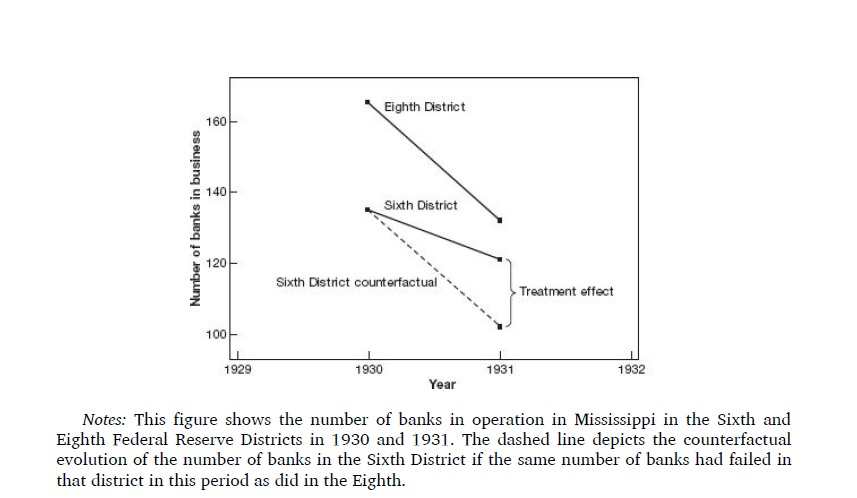
\includegraphics[width=6cm,height=7cm,keepaspectratio]{Figure 5.1} 

\column{.5\textwidth}
\begin{itemize}
	\item dotted line: counterfactual outcome 
	\item shows what would have happened, had they evolved the same way

\end{itemize}

\end{columns}

\end{frame}

%---------------------------------------------------
\begin{frame}
\frametitle{Is there a common trend?}

 \begin{columns}
\column{.45\textwidth}
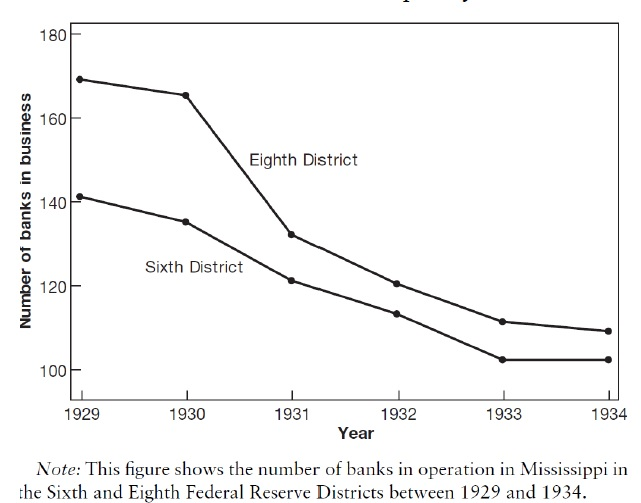
\includegraphics[width=6cm,height=7cm,keepaspectratio]{Figure 5.2} 

\column{.5\textwidth}
\begin{itemize}
	\item long time series on bank activity
	\item before 1930, similar policy
	\item bank failure moved almost in parallel in the two districts
	\item banks declining slightly in both districts
	\item common trends assumption seems valid

\end{itemize}

\end{columns}

\end{frame}

%---------------------------------------------------

\begin{frame}
\frametitle{Adding the Sixth District counterfactual }

 \begin{columns}
\column{.45\textwidth}
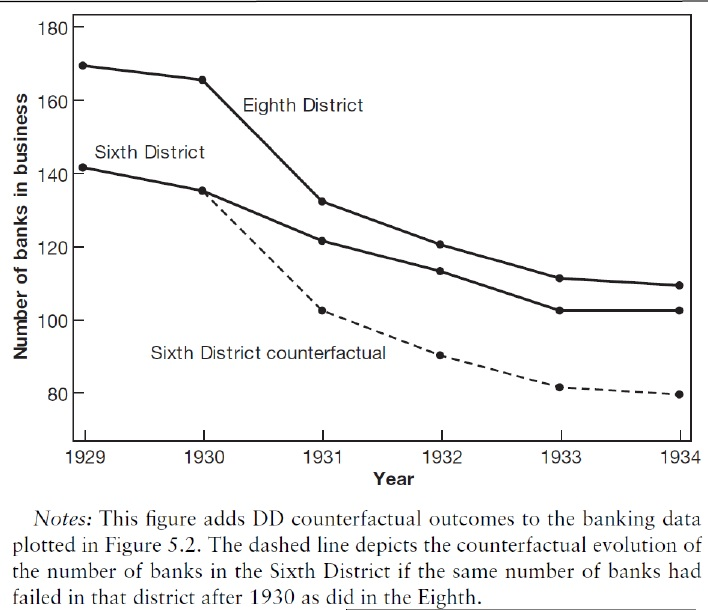
\includegraphics[width=6cm,height=7cm,keepaspectratio]{Figure 5.3} 

\column{.5\textwidth}
\begin{itemize}
	\item counterfactual implied by extrapolating Eight District trends ti the Sixth
	\item in 1931, St.Louis Fed started lending money and the two districts had a similar policy again

\end{itemize}

\end{columns}

\end{frame}

%---------------------------------------------------

\begin{frame}
\frametitle{A Depression Regression}
\begin{itemize}
	\item we will use regression models fit to samples of more than four data points and more than two cross-sectional units
	\item our regession DD recipe contains
		\begin{itemize}
			\item a dummy for the treatment $TREAT_d$ (equals 1 for data points from Sixths Districts)
			\item a dummy for post-treatment periods $POST_t$ (observations from 2931 onward)
			\item the interaction term $TREAT_d~x~POST_t$ (observations in the Sixth District in periods when Fed's response mattered for number of active banks)
		\end{itemize}
	\item what would our regression equation look like?
\end{itemize}

\end{frame}
%------------------------------------------------


\begin{frame}
\frametitle{A Depression Regression}
\begin{itemize}
	\item putting our three ingredients together, we obtain:
	$$Y_d_t = \alpha + \beta TREAT_d + \gamma POST_t + \delta_{rDD} (TREAT_d ~x~POST_t) + e_d_t$$
	\item this sample is constructed by tacking observations from both districts and six available years for each district
	\item $\delta_r_D_D$ is our causal effect of interest
\end{itemize}

\end{frame}
%------------------------------------------------

\begin{frame}
\frametitle{A Depression Regression}
\begin{itemize}
	\item fitting this equation to our 12 observations from Figure 5.2. we get:
	$$Y_d_t = 167 - 29 TREAT_d - 49 POST_t $$
	$$+ 20.5_{rDD} (TREAT_d ~x~POST_t) + e_d_t $$
	\item standard errors $\beta$: 8.8 , $\gamma$: 7.6, $\delta$: 10.7
	\item this suggests that roughly 21 banks were kept alive by Sixth District lending
	\item looking at the standard error for $\delta$, this is a marginally significant result
\end{itemize}

\end{frame}
%------------------------------------------------

\begin{frame}
\frametitle{Did the policy support real economic activity? }

 \begin{columns}
\column{.45\textwidth}
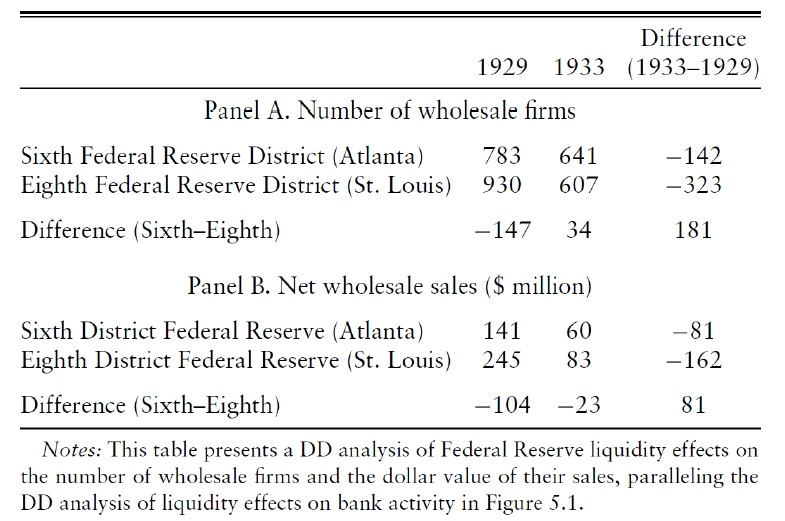
\includegraphics[width=6cm,height=7cm,keepaspectratio]{Table 5.1} 

\column{.5\textwidth}
\begin{itemize}
	\item DD analysis of Fed Reserve liquidity effects on the number of active wholesalers and their sales
	\item the reduction in bank credit in the Eigth District brought wholesale business activity down unlike in the Sixth
	\item as only four-number DD, the evidence for a liquidity treatment effect is weaker than that produced by our larger sample for bank activity

\end{itemize}

\end{columns}

\end{frame}

%---------------------------------------------------



%ab hier aktuell. Chapter 5 by Max on 26.05  %%%%%%%%%%%%%%%%%%%%%%%%%%%%%%%%%%%%%%%%%%%%%%%
%---------------------------------------------------
\section{DiD on the MLDA}

\begin{frame}
\frametitle{DiD on the MLDA}
\begin{itemize}
	\item Alabama lowered its MLDA to 19 in 1975, geographically near Arkansas has had an MLDA of 21.
	\item Did Alabama’s indulgence of its youthful drinkers cost some of them their lives? 
	\item We want to find out by fitting a regression DD model to data on the death rates of 18–20-year-olds from 1970 to 1983. 
	\item The dependent variable is denoted $Y_{st}$, for death rates in state s and year t.
$$Y_{st}=\alpha + \beta~ TREAT_s + \gamma ~POST_t + \sigma_{rDD} (TREAT_s \times POST_t) + \epsilon_{st}$$

\end{itemize}

\end{frame}

%---------------------------------------------------

\begin{frame}
\frametitle{Explaining the regression}
\begin{itemize}
	\item $TREAT_s$ is a dummy variable indicating Alabama. 
	\item $POST_t$ is a dummy indicating years from 1975 onward.
	\item Interaction term $TREAT_s \times POST_t$ indicates Alabama observations from low-drinking-age years. 
	\item The coefficient $\sigma_{rDD}$ captures the effect of an age-19 MLDA on death rates.
\end{itemize}
\end{frame}

%---------------------------------------------------

\begin{frame}
\frametitle{Larger Sample = More Success}
\begin{itemize}
	\item Remember: Larger sample produces more precise results.
	\item So: We should take all districts with different MLDA laws into account.
	\item We swap the single $POST_t$ dummy for a set of dummies indicating each year in the sample, with one omitted as a reference group. 
	\item The coefficients on these dummies, known as time effects, capture temporal changes in death rates that are common to all states.
\end{itemize}


\end{frame}

%---------------------------------------------------

\begin{frame}
\frametitle{Multistate setup}
\begin{itemize}
	\item Multistate setup controls for the differing death rates in each of many states. 
	\item This is accomplished by introducing state effects, a set of dummies for every state in the sample, except for one, which is omitted as a reference group.
	\item A regression DD analysis of data from Alabama, Arkansas, and Tennessee, for example, includes two state effects. 
	\item State effects replace the single $TREAT_s$ dummy included in a two-state (or twogroup) analysis.

\end{itemize}

\end{frame}
%---------------------------------------------------

\begin{frame}
\frametitle{Explaining the regression}
\begin{itemize}
	\item A final complication in this scenario is the absence of a common treatment variable that discretely switches off and on.
	\item We replace $TREAT_d ×POST_t$ with a variable well call $LEGAL_{st}$. 
	\item This variable measures the proportion of 18–20-year-olds allowed to drink in state s and year t. 
	\item In some states, no one under 21 is allowed to drink, while in states with an age-19 MLDA, roughly two-thirds of 18–20-year-olds can drink, and in states with an age-18 MLDA, all 18–20-year-olds can drink

\end{itemize}
\end{frame}

%---------------------------------------------------

\begin{frame}
\frametitle{Explaining the regression}
	\begin{itemize}
		\item Multistate regression DD model looks like: 
\small$$Y_{st}=\alpha +\sigma_{rDD} LEGAL_{st} + \sum_{k=Alaska}^{Wyoming}\beta_k~ STATE_{ks} + \sum_{j=1971}^{1983}\gamma_j~YEAR_{jt} + \epsilon_{st}$$
		\item Here every state but one (the reference state) gets its own dummy variable, indexed by the subscript k for state k. 
		\item Observations from California, for example, have $STATE_{CA}$, s switched on, and all other state dummies switched off.

	\end{itemize}

\end{frame}
%---------------------------------------------------

\begin{frame}
\frametitle{Explaining the regression}
	\begin{itemize}
		\item $\beta_k$, are the coefficients on the state dummies. 
		\item For example, the California state effect, $\beta_{CA}$ is the coefficient on $STATE_{CA,s}$
		\item Every state except the reference state, the one omitted when constructing state dummies, has a state effect in this equation.
		\item Same goes for year effects, e.g. The 1975 year effect, $\gamma_{1975}$, is the coefficient on $YEAR{1975, t}$.
\end{itemize}

\end{frame}
%---------------------------------------------------

\begin{frame}
\frametitle{Explaining the regression}
	\begin{itemize}
		\item Our multistate MLDA analysis uses a data set with 14 years and 51 states for a total of 714 observations. 			
		\item This data structure is called a state-year panel.
		\item The state effects control for fixed differences between states (for example, fatal car accidents are more frequent, on average, in rural states with high average travel speeds). 
		\item The time (year) effects in this equation control for trends in death rates that are common to all states (due, for example, to national trends in drinking or vehicle safety).
		\item This equation attributes changes in mortality within states to changes in $LEGAL_{st}$.

	\end{itemize}
\end{frame}

%--------------------------------------

\begin{frame}
\frametitle{Effect of different MLDA on death}
	
\begin{columns}
\column{.5\textwidth}
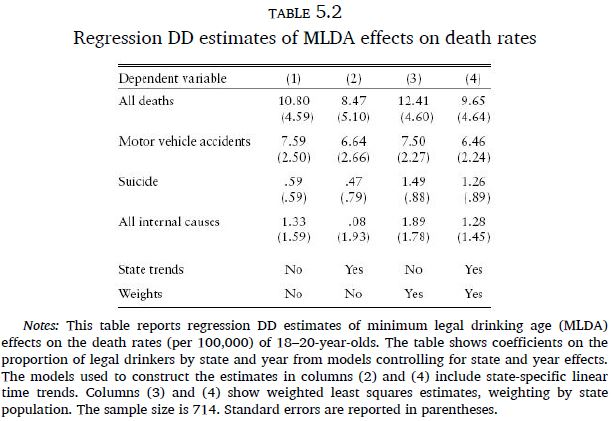
\includegraphics[width=6.3cm,height=7.5cm,keepaspectratio]{Table 5.2} 

\column{.45\textwidth}
\begin{itemize}
	\item Legal alcohol access caused about 11 additional deaths per 100,000 18–20-year-olds, of which seven or eight deaths were the result of motor vehicle accidents.
	\item Generates little evidence of an effect of legal drinking on deaths from internal causes.
\end{itemize}

\end{columns}


\end{frame}



%---------------------------------------------------

\begin{frame}
\frametitle{Always common trends?}
	\begin{itemize}
		\item Samples that include many states and years allow us to relax the common trends assumption, that is, to introduce a degree of nonparallel evolution in outcomes between states in the absence of a treatment effect.
		\item Such a regression looks like: 
		\begin{flalign*}
	Y_{st}=\alpha +\sigma_{rDD} LEGAL_{st} + \sum_{k=Alaska}^{Wyoming}\beta_k~ STATE_{ks} \\
				+ \sum_{j=1971}^{1983}\gamma_j~YEAR_{jt} + \sum_{k=Alaska}^{Wyoming} \theta_k (STATE_{ks} \times t) + \epsilon_{st}
		\end{flalign*}
		\item In the absence of a treatment effect, death rates in state k deviate from common year effects by following the linear trend captured by the coefficient $\theta_k$.

	\end{itemize}

\end{frame}


%---------------------------------------------------
\begin{frame}
\frametitle{Uncommon Trends}
	\begin{columns}
\column{.45\textwidth}
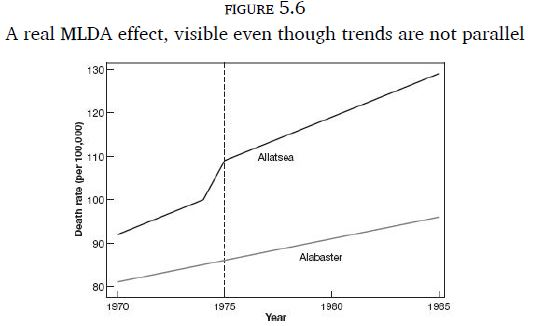
\includegraphics[width=5cm,height=6cm,keepaspectratio]{Figure 5.6} 

\column{.7\textwidth}
\begin{itemize}
	\item Regression DD captures treatment effects with of uncommon trends. 
	\item Death rates in Allatsea increase more steeply than in Alabaster.
	\item But the Allatsea increase is especially steep from 1974 to 1975, when Allatsea lowered its
MLDA. 
	\item The coefficient on $LEGAL_{st}$ picks this up, while the model allows for the fact that death rates in different states were on different trajectories from the get-go.
\end{itemize}

\end{columns}
\end{frame}


%---------------------------------------------------
\begin{frame}
\frametitle{Controls}
	\begin{itemize}
		\item But: We should control for other factors too.
		\item Important consideration in research on alcohol is the price of a drink. 
	  \item Taxes are the most powerful tool the government uses to affect the price.
		\item States might raise tax rates at the same time that they increase their MLDA.

	\end{itemize}

\end{frame}



%---------------------------------------------------
\begin{frame}
\frametitle{With Controls}

 \begin{columns}
\column{.45\textwidth}
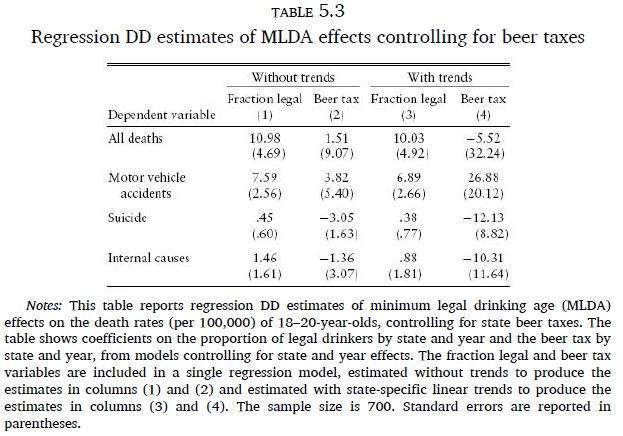
\includegraphics[width=6cm,height=7cm,keepaspectratio]{Table 5.3} 

\column{.5\textwidth}
\begin{itemize}
	\item Generate MLDA estimates similar to those without such controls.
	\item The beer tax estimates from models that include state trends are especially noisy.

\end{itemize}

\end{columns}

\end{frame}


%---------------------------------------------------

\begin{frame}
\frametitle{Weighted least squares (WLS)}
	\begin{itemize}
		\item States are not created equal: some, like Texas and California, are bigger than most countries, while others, like Vermont and Wyoming, have populations smaller than those of many American cities.
		\item Solution: Use weighted least squares (WLS)
		\item Standard OLS estimator fits a line by minimizing the sample average of squared residuals, with each squared residual getting equal weight in the sum.
		\item WLS weights each term in the residual sum of squares by population size or some other researcher-chosen weight.
		\item Capture a weighted average of effects for the groups or cells represented in our data

	\end{itemize}

\end{frame}

%---------------------------------------------------
\section{In a nutshell}
\begin{frame}
\frametitle{In a nutshell}
	\begin{itemize}
		\item Treatment and control groups may differ in the absence of treatment, yet move in parallel. 
		\item This pattern opens the door to DD estimation of causal effects.
		\item Comparing changes instead of levels, we eliminate fixed differences between groups that might otherwise generate omitted variables bias.
		\item It has power and flexibility, in a state-year panel we need only control for state and year effects.
		\item Important: Parallel trends, the claim that in the absence of treatment, treatment and control group outcomes would move in parallel (Although we can control for nonparallel trends).


	\end{itemize}

\end{frame}


%---------------------------------------------------
\section{Appendix}

\begin{frame}
\frametitle{Serial correlations}
	\begin{itemize}
		\item Regression DD is a special case of estimation with panel data. 
		\item A state-year panel consists of repeated observations on states over time. 
		\item The repetitive structure of such data sets raises special statistical problems.
		\item Economic data of this sort typically exhibit a property called serial correlation.
		\item Serially correlated data are persistent, meaning the values of variables for nearby periods are likely to be similar.
		\item When the dependent variable in a regression is serially correlated, the residuals from any regression model explaining this variable are often serially correlated as well.

	\end{itemize}

\end{frame}

%---------------------------------------------------
\begin{frame}
\frametitle{Serial correlations}
	\begin{itemize}
		\item Serial correlation is a deviation from randomness, with the important consequence that each new observation in a serially correlated time series contains less information than would be the case if the sample were random.
		\item The formula used in this case is the clustered standard errors formula
		\item Clustering allows for correlated data within researcher defined clusters. 

	\end{itemize}

\end{frame}

%---------------------------------------------------

\begin{frame}
\frametitle{Clustered standard errors}
	\begin{itemize}
		\item In contrast with the assumption that all data are randomly sampled, the formula for clustered standard errors requires only that clusters be sampled randomly, with no random sampling
		\item Assumption invoked for what’s inside them.
		\item In principle, clustering solves any sort of dependence problem in your data 
		\item Especially useful for panel data
		\item But: Large standard errors as a result
	\end{itemize}

\end{frame}

%----------------------------------------------------------------------------------------

\begin{frame}
\Huge{\centerline{Thank you very much for listening}}
\end{frame}

%----------------------------------------------------------------------------------------

\end{document} 